\documentclass{article}
\usepackage{tikz}
\usetikzlibrary{automata,positioning}

\begin{document}

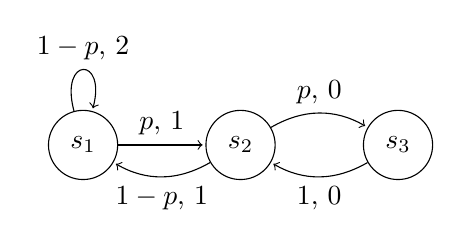
\begin{tikzpicture}[shorten >=1pt,node distance=2cm,on grid,auto]
    \node[state] (s1) {$s_1$};
    \node[state] (s2) [right=of s1] {$s_2$};
    \node[state] (s3) [right=of s2] {$s_3$};

    \path[->]
        (s1) edge [loop above] node {$1-p$, $2$} ()
             edge node {$p$, $1$} (s2)
        (s2) edge [bend left] node {$p$, $0$} (s3)
             edge [bend left] node {$1-p$, $1$} (s1)
        (s3) edge [bend left] node {$1$, $0$} (s2);
\end{tikzpicture}

\end{document}